
% Slideshow, written by Brent Baccala, for a summary lecture of calculus

\documentclass{beamer}
\usetheme{Madrid}

\title{Large Language Models}
\author{Brent Baccala}
\institute{\tt cosine@freesoft.org}
%% \date{February 8, 2023}

\setbeamertemplate{footline}{}
\beamertemplatenavigationsymbolsempty

\usepackage{amsmath}
\usepackage{tabularx}

\usepackage{breqn}

\usepackage{xcolor}
\usepackage{comment}
\usepackage{graphicx}

\usepackage{tabularx}

\usepackage{fancyvrb}

\usepackage{tikz}
\usetikzlibrary{positioning}
\usetikzlibrary{fit}
\usetikzlibrary{backgrounds}
\usetikzlibrary{angles,quotes,3d}
\usetikzlibrary{decorations.pathreplacing}
\usetikzlibrary{calc,intersections}
\usepackage{tikz-3dplot}

\usepackage{pgfplots}
\pgfplotsset{compat=1.16}

\usepackage{adjustbox}

\begin{document}


\begin{frame}
\titlepage
\begin{block}{Abstract}
A survey of Large Language Models
\end{block}
\end{frame}

\begin{frame}
\begin{itemize}
\item The traditional way of diagraming a neural network
\item A different way of looking at it (staircase)
\item Alternating linear and non-linear layers
\item How does a LLM work? (the concept of a token)
\item bfloat16
\end{itemize}
\end{frame}

\begin{frame}
\frametitle{Floating Point Formats}
\begin{center}
% IEEE half-precision 16-bit float
% \begin{tikzpicture}[node distance=0pt,outer sep=0pt]
%
% % Row 1
% \node [draw, text width=1cm, align=center, fill=white] (sign) {sign};
% \node [draw, text width=4cm, align=center, fill=white, right=of sign] (exponent) {exponent (5 bit)};
% \node [draw, text width=6cm, align=center, fill=white, right=of exponent] (fraction) {fraction (10 bit)};
%
% % Row 2
% \node [draw, text width=1cm, align=center, fill=white, below=of sign] (sign_val) {0};
% \node [draw, text width=4cm, align=center, fill=white, right=of sign_val] (exponent_val) {0 \quad 0 \quad 1 \quad 1 \quad 0};
% \node [draw, text width=6cm, align=center, fill=white, right=of exponent_val] (fraction_val) {0 0 0 0 0 0 0 0 0 0};
%
% \end{tikzpicture}
%
% \vskip 12pt

IEEE single-precision 32-bit float (most CPUs)

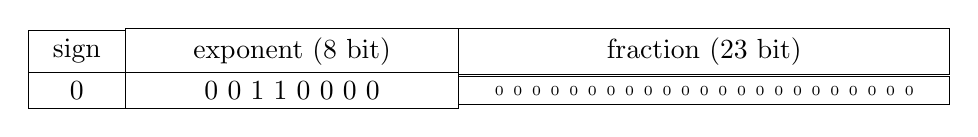
\begin{tikzpicture}[node distance=0pt,outer sep=0pt]

% Row 1
\node [draw, text width=1cm, align=center, fill=white] (sign) {sign};
\node [draw, text width=4cm, align=center, fill=white, right=of sign] (exponent) {exponent (8 bit)};
\node [draw, text width=6cm, align=center, fill=white, right=of exponent] (fraction) {fraction (23 bit)};

% Row 2
\node [draw, text width=1cm, align=center, fill=white, below=of sign] (sign_val) {0};
\node [draw, text width=4cm, align=center, fill=white, right=of sign_val] (exponent_val) {0 0 1 1 0 0 0 0};
\node [draw, text width=6cm, align=center, fill=white, right=of exponent_val] (fraction_val) {\tiny 0 0 0 0 0 0 0 0 0 0 0 0 0 0 0 0 0 0 0 0 0 0 0};

\end{tikzpicture}

bfloat16 (most GPUs and AVX-512 CPUs)

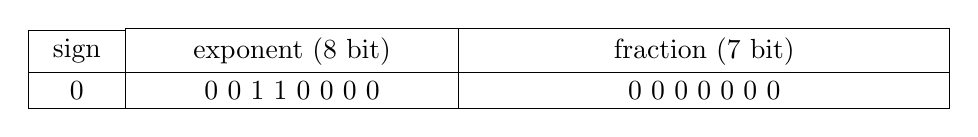
\begin{tikzpicture}[node distance=0pt,outer sep=0pt]

% Row 1
\node [draw, text width=1cm, align=center, fill=white] (sign) {sign};
\node [draw, text width=4cm, align=center, fill=white, right=of sign] (exponent) {exponent (8 bit)};
\node [draw, text width=6cm, align=center, fill=white, right=of exponent] (fraction) {fraction (7 bit)};

% Row 2
\node [draw, text width=1cm, align=center, fill=white, below=of sign] (sign_val) {0};
\node [draw, text width=4cm, align=center, fill=white, right=of sign_val] (exponent_val) {0 0 1 1 0 0 0 0};
\node [draw, text width=6cm, align=center, fill=white, right=of exponent_val] (fraction_val) {0 0 0 0 0 0 0};

\end{tikzpicture}

\vskip 12pt

\end{center}

Source: Wikipedia, {\it bfloat16 floating-point format}
\end{frame}

\begin{frame}
\frametitle{Heatmap token representations}
\includegraphics[width=0.3\textwidth]{14614.png}
\includegraphics[width=0.3\textwidth]{248.png}
\includegraphics[width=0.3\textwidth]{772.png}
\includegraphics[width=0.3\textwidth]{3020.png}
\includegraphics[width=0.3\textwidth]{4169.png}
\end{frame}

\begin{frame}[fragile]
\frametitle{Heatmap token representations}
After extracting the tokens to {\tt words.torch}:
\tiny\begin{verbatim}
import torch
import seaborn as sns
import matplotlib.pyplot as plt

from transformers import AutoTokenizer

tokenizer = AutoTokenizer.from_pretrained('tiiuae/falcon-40b-instruct')

with open('words.torch', 'rb') as f:
    words=torch.load(f)

def tword(num):
    return words[num].float().view(64,71)

for token in tokenizer.tokenize("Print the first ten numbers"):
    id = tokenizer.convert_tokens_to_ids(token)
    plt.clf()
    sns.heatmap(tword(id).numpy(), center=0, cmap='coolwarm')
    plt.title(f'{id}: {token}', fontsize=20)
    plt.savefig(f'{id}.png')

\end{verbatim}
\end{frame}

\begin{frame}
\begin{itemize}
\item Git / Git Large Files Extension
\item Why it warns about running untrusted code
\item What is a tensor
\item Basic structure of Hugging Face library / custom code
\item How to read the falcon python code
\item How to do attention by hand
\item How to split an LLM across multiple nodes by splitting the loop
\item How to split an LLM across multiple nodes by splitting the tensors
\item How training works - additional values need to be tracked for each parameter (ADAM)
\end{itemize}
\end{frame}

\begin{frame}[fragile]
\frametitle{Falcon's main inference loop}
\tiny\begin{verbatim}
class RWModel(RWPreTrainedModel):
    def forward(...):

        ...

        for i, (block, layer_past) in enumerate(zip(self.h, past_key_values)):

            if output_hidden_states:
                all_hidden_states = all_hidden_states + (hidden_states,)

            outputs = block(
                hidden_states,
                layer_past=layer_past,
                attention_mask=causal_mask,
                head_mask=head_mask[i],
                use_cache=use_cache,
                output_attentions=output_attentions,
                alibi=alibi,
            )

            hidden_states = outputs[0]
            if use_cache is True:
                presents = presents + (outputs[1],)

            if output_attentions:
                all_self_attentions = all_self_attentions + (outputs[2 if use_cache else 1],)

\end{verbatim}
\end{frame}

\begin{frame}[fragile]
\frametitle{Split an LLM across multiple nodes by splitting the loop (functions to send/recv tensors)}
\tiny\begin{verbatim}
import torch.distributed as dist

dtype_to_int = {
    torch.float32: 0,
    torch.float64: 1,
    torch.float16: 2,
    torch.uint8: 3,
    torch.int8: 4,
    torch.int16: 5,
    torch.int32: 6,
    torch.int64: 7,
    torch.bool: 8
}

int_to_dtype = {value: key for key, value in dtype_to_int.items()}

def send_tensor(tensor, dst):
    length = torch.tensor([len(tensor.shape), dtype_to_int[tensor.dtype]], dtype=torch.long)
    shape = torch.tensor(tensor.shape, dtype=torch.long)
    dist.send(length, dst=dst)
    dist.send(shape, dst=dst)
    dist.send(tensor, dst=dst)

def recv_tensor(src):
    length = torch.zeros(2, dtype=torch.long)
    dist.recv(length, src=src)
    shape = torch.zeros(length[0], dtype=torch.long)
    dist.recv(shape, src=src)
    tensor = torch.empty(tuple(shape), dtype=int_to_dtype[int(length[1])])
    dist.recv(tensor, src=src)
    return tensor

\end{verbatim}
\end{frame}

\begin{frame}[fragile]
\frametitle{Split an LLM across multiple nodes by splitting the loop (functions to send/recv state)}
\tiny\begin{verbatim}
def send_state(dst, use_cache, alibi, head_mask, output_hidden_states, output_attentions, hidden_states, past_key_values, causal_mask, all_hidden_states, all_self_attentions):

    use_alibi = alibi is not None
    use_past_key_values = past_key_values[0] is not None
    use_head_mask = head_mask[0] is not None

    flags = torch.tensor([use_alibi, use_cache, use_past_key_values, use_head_mask,
                          output_hidden_states, output_attentions], dtype=torch.bool)

    send_tensor(flags, dst=dst)
    send_tensor(hidden_states, dst=dst)
    if use_past_key_values:
        for t in past_key_values:
            send_tensor(t, dst=dst)
    send_tensor(causal_mask, dst=dst)
    if alibi:
        send_tensor(alibi, dst=dst)
    if use_head_mask:
        send_tensor(head_mask, dst=dst)
    if output_hidden_states:
        for t in all_hidden_states:
            send_tensor(t, dst=dst)
    if output_attentions:
        for t in all_self_attentions:
            send_tensor(t, dst=dst)
\end{verbatim}
\end{frame}

\begin{frame}[fragile]
\frametitle{Split an LLM across multiple nodes by splitting the loop (load only a subset of the tensors)}
\tiny\begin{verbatim}
class RWModel(RWPreTrainedModel):
    def __init__(self, config: RWConfig):

       ...

       # Transformer blocks (original code)
       # self.h = nn.ModuleList([DecoderLayer(config) for _ in range(config.num_hidden_layers)])

       # Transformer blocks (split across multiple nodes)
       self.h = nn.ModuleList([DecoderLayer(config)
                               if i * args.world_size // config.num_hidden_layers == args.rank
                               else None
                               for i in range(config.num_hidden_layers)])
\end{verbatim}
\end{frame}

\begin{frame}[fragile]
\frametitle{Split an LLM across multiple nodes by splitting the loop (load only a subset of the tensors)}
\tiny\begin{verbatim}
class RWModel(RWPreTrainedModel):
    def forward(
        self,
        input_ids: Optional[torch.LongTensor] = None,
        past_key_values: Optional[Tuple[Tuple[torch.Tensor, torch.Tensor], ...]] = None,
        attention_mask: Optional[torch.Tensor] = None,
        head_mask: Optional[torch.LongTensor] = None,
        inputs_embeds: Optional[torch.LongTensor] = None,
        use_cache: Optional[bool] = None,
        output_attentions: Optional[bool] = None,
        output_hidden_states: Optional[bool] = None,
        return_dict: Optional[bool] = None,
        **deprecated_arguments,
    ) -> Union[Tuple[torch.Tensor, ...], BaseModelOutputWithPastAndCrossAttentions]:

        ...

        send_state(1, use_cache, alibi, head_mask, output_hidden_states, output_attentions, hidden_states, past_key_values, causal_mask, all_hidden_states, all_self_attentions)

        # Wait for it to go around the distributed nodes and come back

        src = builtins.args.world_size - 1

        (use_cache, alibi, head_mask, output_hidden_states, output_attentions, hidden_states, past_key_values, causal_mask, all_hidden_states, all_self_attentions) = recv_state(src, len(self.h))
\end{verbatim}
\end{frame}

\begin{frame}[fragile]
\frametitle{Split an LLM across multiple nodes by splitting the loop (the startup code)}
%% The startup code --
The program now accepts {\tt --world-size} and {\tt --rank}
arguments that tell it, respectively, how many parallel processes are running
in total, and which of those processes is the current one.

All processes except rank 0 then run a loop where they wait to receive a state
vector, run it through the layers of the model loaded on that process, and
pass it on to the next process.
\tiny\begin{verbatim}
import torch.distributed as dist

init_method = 'tcp://c200-1:23457'

parser = argparse.ArgumentParser(description="Run inference with falcon-40b-instruct")

parser.add_argument("--rank", type=int, default=0, help="Rank of the current process")
parser.add_argument("--world-size", type=int, default=1, help="Total number of processes")

args = parser.parse_args()
builtins.args = args

dist.init_process_group(backend='gloo', init_method=init_method, rank=args.rank, world_size=args.world_size)

if args.rank > 0:
    src = args.rank - 1
    dst = (args.rank + 1) % args.world_size
    # we keep waiting for a job to run through the arg.rank'th part of the model
    while True:
        (use_cache, alibi, head_mask, output_hidden_states, output_attentions, hidden_states, past_key_values, causal_mask, all_hidden_states, all_self_attentions) = recv_state(src, len(model.transformer.h))

        for i, (block, layer_past) in enumerate(zip(model.transformer.h, past_key_values)):
\end{verbatim}
\end{frame}

\begin{frame}
Disadvantage of this approach
\begin{itemize}
\item all nodes except one are idle at any one time
\end{itemize}

\vskip 12pt

A better approach
\begin{itemize}
\item parallelize so that all nodes run simultaneously
\end{itemize}

\vskip 12pt

How can this be done?

\end{frame}

\begin{frame}[fragile]
\frametitle{A Multilayer Perceptron in Python}
{\tiny\begin{verbatim}
class MLP(nn.Module):
    def __init__(self, config: RWConfig):
        super().__init__()
        hidden_size = config.hidden_size

        self.dense_h_to_4h = Linear(hidden_size, 4 * hidden_size, bias=config.bias)
        self.act = nn.GELU()
        self.dense_4h_to_h = Linear(4 * hidden_size, hidden_size, bias=config.bias)
        self.hidden_dropout = config.hidden_dropout

    def forward(self, x: torch.Tensor) -> torch.Tensor:
        x = self.act(self.dense_h_to_4h(x))
        x = self.dense_4h_to_h(x)
        return x
\end{verbatim}}
Source: falcon {\tt modelling_RW.py}
\end{frame}

\begin{frame}
\frametitle{Parallelizing the MLP across multiple nodes}

\begin{itemize}
\item {\tt Linear} is just a matrix (tensor) multiplication
\item Split the {\tt Linear} tensors into slices, one for each node
\item {\tt torch.distributed} has a Remote Procedure Call (RPC) mechanism
\item figure how to do distributed training
\end{itemize}
\end{frame}

\end{document}
